\documentclass[pdf]{beamer}

\usepackage{amsmath}
\usepackage{amsfonts}

\usepackage{graphics,graphicx,subfigure,color}

\usepackage{tikz} % graphical models
\usetikzlibrary{chains,fit,shapes}
\usetikzlibrary{bayesnet}


\mode<presentation>{}

\title{Extended Topic Models with Etymological Roots}

\author{G\" okhan \c Capan, Ali Caner T\" urkmen}
\begin{document}
	
\begin{frame}
	\titlepage
\end{frame}

\begin{frame}{Reminder: Topic Models}
	
	\begin{itemize}
		\item {\em Unsupervised} learning, recover \emph{latent} topics in documents
		\item Can be thought of as {\em clustering}.
		\item {\bf Key Ideas:} 
			\begin{itemize}
			\item Topics lead to distinct word distributions. 
			\item  A document includes words from multiple topics (in contrast with clustering)
			\end{itemize}
	\end{itemize}
\end{frame}


\begin{frame}{LDA - Generative Model}	
	\begin{itemize}
		\item For each document;
		\begin{itemize}
			\item Topic proportions vector is drawn ($\theta \sim Dirichlet(\alpha)$)
			\item For each word in the document
			\begin{itemize}
				\item A topic is drawn from topic proportions ($z_i \sim Multinomial(\theta)$)
				\item The word is drawn from topic ($w_i \sim Multinomial(\beta_{z_i})$)
			\end{itemize}
		\end{itemize}
	\end{itemize}
\end{frame}


\begin{frame}{LDA - Bayesian Network Representation}
	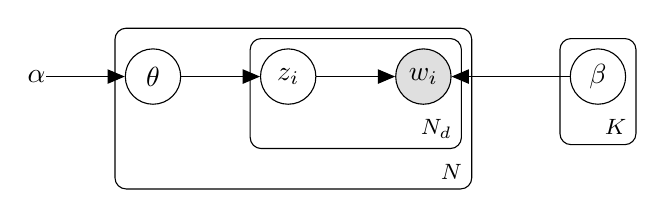
\begin{tikzpicture}
	  \node[latent] (z) {$z_i$} ; %
	  \node[obs, right = of z] (w) {$w_i$};
          \node[latent, left=of z] (theta) {$\theta$} ; %
          \node[const, left=of theta](alpha){$\alpha$};
          \node[latent, right=1.5 of w] (beta) {$\beta$};
        
          \edge {theta} {z} ; %
          \edge {z} {w} ;
          \edge {beta}{w} ;
          \edge {alpha}{theta}
          
          \plate {words}{
          	(z)
		(w)
	  }{$N_d$}
	  
          \plate {docs} {
          	(theta)
		(words)
          }{$N$}
          
          \plate {topicwords}{
          	(beta)
	 }{$K$}
    
	\end{tikzpicture}
	\hspace{5cm}
	\begin{itemize}
		\item Note the difference with document clustering ($z$ is outside of the plate in that case, each word of a document comes from a single cluster), which is referred to as \textit{mixture of unigrams}
	\end{itemize}
\end{frame}

\begin{frame}{LDA - Generative Model}
	\begin{itemize}
		\item $\theta$ is like a histogram, a proportions vector representing membership of document to topics
		\item Words come from topics, and word-topic memberships from topic histograms
	\end{itemize}
\end{frame}


\begin{frame}{Multi Modal LDA Model}
	\begin{itemize}
		\item A topic can give rise to other (than words) observed phenomena
		\item We hypothesized to utilize etymological roots of words
		\begin{itemize}
			\item A word is paired with an etymological root
			\item The (per word) topic membership also generates the etymological root
		\end{itemize}
	\end{itemize}
\end{frame}

\begin{frame}{Graphical Model}
	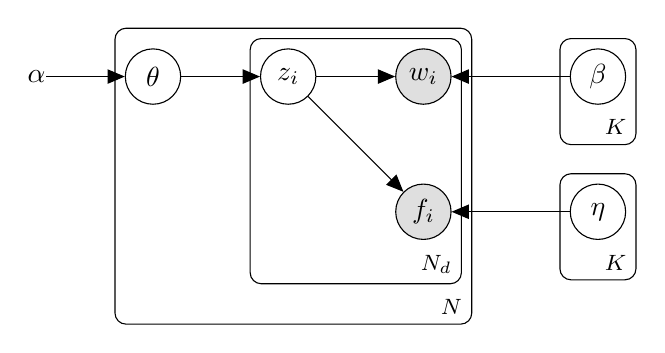
\begin{tikzpicture}
	  \node[latent] (z) {$z_i$} ; %
	  \node[obs, right = of z] (w) {$w_i$};
	  \node[obs, below = of w] (f) {$f_i$};
          \node[latent, left=of z] (theta) {$\theta$} ; %
          \node[const, left=of theta](alpha){$\alpha$};
          \node[latent, right=1.5 of w] (beta) {$\beta$};
          \node[latent, right=1.5 of f] (eta) {$\eta$};
        
          \edge {theta} {z} ; %
          \edge {z} {w} ;
          \edge {z} {f};
          \edge {beta}{w} ;
          \edge {eta}{f}
          \edge {alpha}{theta};
          
          \plate {words}{
          	(z)
		(w)
		(f)
	  }{$N_d$}
	  
          \plate {docs} {
          	(theta)
		(words)
          }{$N$}
          
          \plate {topicwords}{
          	(beta)
	 }{$K$}
	\plate{topicfeatures}{
	 	(eta)
	}{$K$}
	\end{tikzpicture}
\end{frame}

\begin{frame}{Learning}
	\begin{itemize}
		\item Variational EM
		\item Iterate:
		\begin{itemize}
			\item For each document d
				\begin{itemize}
					\item Approximate $P(\theta_d, z_d|w_d, \beta, \eta)$ with $q(\theta|\gamma_d) \prod_{n=1}^{N_d}(z_n|\phi_n)$
				\end{itemize}
			\item Find maximum likely $\beta$ and $\eta$
		\end{itemize}
	\end{itemize}
\end{frame}

\begin{frame}{Mean Field Approximation: Unimodal Case}
	\begin{itemize}
		\item Variational updates:
	\end{itemize}
	\begin{equation*}
		\phi_{ni}^{(t)} \gets \beta_{i w_n} \exp\left[\psi\left(\gamma_{i}^{(t-1)}\right) - \psi\left({\sum_{j=1}^k \gamma_j^{(t-1)}}\right)\right]
	\end{equation*}
	
	\begin{equation*}
		\gamma_i^{(t)}\gets \alpha_i + \sum_{n=1}^{N_d} \phi_{ni}^{(t)}
	\end{equation*}
	\begin{itemize}
		\item This is done by \textit{every document and until convergence}
	\end{itemize}

\end{frame}

\begin{frame}{Mean Field Approximation: Multimodal Case}
	\begin{itemize}
		\item Variational updates:
	\end{itemize}
	\begin{equation*}
		\phi_{ni}^{(t)} \gets \eta_{i f_n} \beta_{i w_n} \exp\left[\psi\left(\gamma_{i}^{(t-1)}\right) - \psi\left({\sum_{j=1}^k \gamma_j^{(t-1)}}\right)\right]
	\end{equation*}
	
	\begin{equation*}
		\gamma_i^{(t)}\gets \alpha_i + \sum_{n=1}^{N_d} \phi_{ni}^{(t)}
	\end{equation*}
	\begin{itemize}
		\item Note the extra term
	\end{itemize}

\end{frame}

\begin{frame}{Implementation}
	\begin{itemize}
		\item {\bf Multi-core:} Updating per-document topic histograms (inference step) can be done in parallel. 
		\item {\bf C when necessary:} Implementation is in Python, Cython when necessary
		\item {\bf High performant:} In the uni-modal case, comparable in performance with popular ML libraries (and offers extra features).
		\item {\bf Open:} Ask me if you want to use while we are trying to open it publicly
	\end{itemize}
\end{frame}


\begin{frame}{Data Set}
	
	\begin{itemize}
		\item {\bf Data Set:} News articles sampled from Anadolu Agency website. 1337 documents, from 6 categories: \textit{yasam, politika, spor, turkiye, dunya, ekonomi}
		\item {\bf Preprocessing:} Words that appear in more than 60\% of the documents, less than 5 of them, or those that appear in the Text2ARFF function words list by YTU Kemik Group were ignored (vocabulary size 6226)
	\end{itemize}
	
\end{frame}

\begin{frame}{Getting Etymological Roots}
	
	\begin{itemize}
		\item {\bf TR Wiktionary:} Aggressively match the words in the vocabulary to the Wiktionary lookup (previously crawled)
		\item {\bf Procedure:}
		\begin{itemize}
			\item try to match the word to the etymology lookup
			\item repeat while no hit:
			\begin{itemize}
				\item discard the last letter of the word and try to match again
			\end{itemize}
			\item until there are four letters left
		\end{itemize}
	\end{itemize}
	
\end{frame}

\begin{frame}{Getting Etymological Roots}
	
	\begin{itemize}
		\item TR Wiktionary is poor
		\item We manually tagged them using {\bf Nisanyan Sozluk}
		\item We omitted \textit{Proper Nouns} 
	\end{itemize}
	
\end{frame}

\begin{frame}{Getting Etymological Roots}
	
	\begin{tabular}{c|c}
		Turkish&3397\\
		Arabic&1235\\
		French&486\\
		Farsi&183\\
		English&69\\
		Italian&61\\
		Greek&28\\
		Unassigned&766\\
	\end{tabular}
	
\end{frame}


\begin{frame}{Experimental Results}
	Probability of a word (with variationally computed topic histogram for the including document):
	\begin{equation*}
	 	P(w) = \int \sum_z p(w|z) p(z|\theta)q(\theta)d\theta
	\end{equation*}
	\begin{itemize}
		\item We computed per-word perplexity using the above probability computation for different values of number of topics
	\end{itemize}
	
\end{frame}

\begin{frame}{Perplexity: Unimodal Case}
\begin{figure}
\label{fig:perpuni}
\includegraphics*[width=\textwidth]{perplex-uni.pdf}
\end{figure}
\end{frame}

\begin{frame}{Perplexity: Multimodal Case}
\begin{figure}
\label{fig:perpmulti}
\includegraphics*[width=\textwidth]{perplex-mm.pdf}
\end{figure}
\end{frame}

\begin{frame}{Further Experiments}
	\begin{itemize}
		\item	Assuming (for a moment) documents are of the top clusters they are assigned, we can compare the clustering result with the actual categories 
		\item Two metrics used: Adjusted Rand Index, Adjusted Mutual Information
	\end{itemize}
	
\end{frame}

\begin{frame}{Evaluation of Clusters}
\begin{figure}
\label{fig:ARI}
\includegraphics*[width=\textwidth]{ARI.pdf}
\end{figure}
\end{frame}
	
\begin{frame}{Evaluation of Clusters}
	\begin{figure}
	\label{fig:AMI}
	\includegraphics*[width=\textwidth]{AMI.pdf}
	\end{figure}
\end{frame}

\begin{frame}{Topic Summaries}
\begin{itemize}
\item We can get a sense of what topics represent: as probability distributions (multinomial) over words
\item Further, we can explore how etymologycal roots change across topics
\item Note that in the sequel, only words with length $\geq 5$ are shown
\end{itemize}
\end{frame}

\begin{frame}{Topic Summaries: Unimodal}
\begin{figure}
\label{fig:sum}
\includegraphics*[width=\textwidth]{topics1.jpeg}
\end{figure}
\end{frame}

\begin{frame}{Topic Summaries: Multimodal}
\begin{figure}
\label{fig:sum21}
\includegraphics*[width=\textwidth]{topics2-1.jpeg}
\end{figure}
\end{frame}

\begin{frame}{Topic Summaries: Multimodal (contd)}
\begin{figure}
\label{fig:sum22}
\includegraphics*[width=\textwidth]{topics2-2.jpeg}
\end{figure}
\end{frame}

\begin{frame}{Topic Summaries: Multimodal}
\begin{tabular}{c|c}
Root&Seen as Top Etymology\\
\hline
Arabic&12\\
Turkish&6\\
Italian&1\\
Farsi&1
\end{tabular}
\end{frame}

\begin{frame}{Discussion}
\begin{itemize}
\item LDA with etymological roots can end up with closer top clusters to the actual categories
\item Etymologies were more mixed than previously assumed
\item Proper nouns do not get etymology tags and they tend to cluster in a topic of their own
\end{itemize}
\end{frame}

\begin{frame}{Implementation Discussion}
\begin{itemize}
\item Multimodal LDA implementation is more general
\item Any discrete word-level `side' feature can be used
\item We further provide \textit{predicting the next-word} functionality
\end{itemize}
\end{frame}

\begin{frame}{LDA Discussion}
\begin{itemize}
\item LDA is more general than topic modeling, and can be applied to many problems with mixed-membership assumption and discrete observations
\item Example: Collaborative Filtering (with multimodal extension to item characteristics)
\end{itemize}
\end{frame}

\begin{frame}{}
	
	Thank You!
	
	\hspace{5cm}
	
	gokhan.capan [at] boun.edu.tr
	
	caner.turkmen [at] boun.edu.tr
	
\end{frame}
\bibliography{final}{}
\bibliographystyle{apalike}


\end{document}